\section{RTL Implementation}

\subsection{Bộ thực hiện tính giá trị trung bình của mảng (PACM\_UNIT)}

\subsubsection{Bộ tính cộng số thực (BFP16\_add)}

\begin{figure}[H]
	\centering
	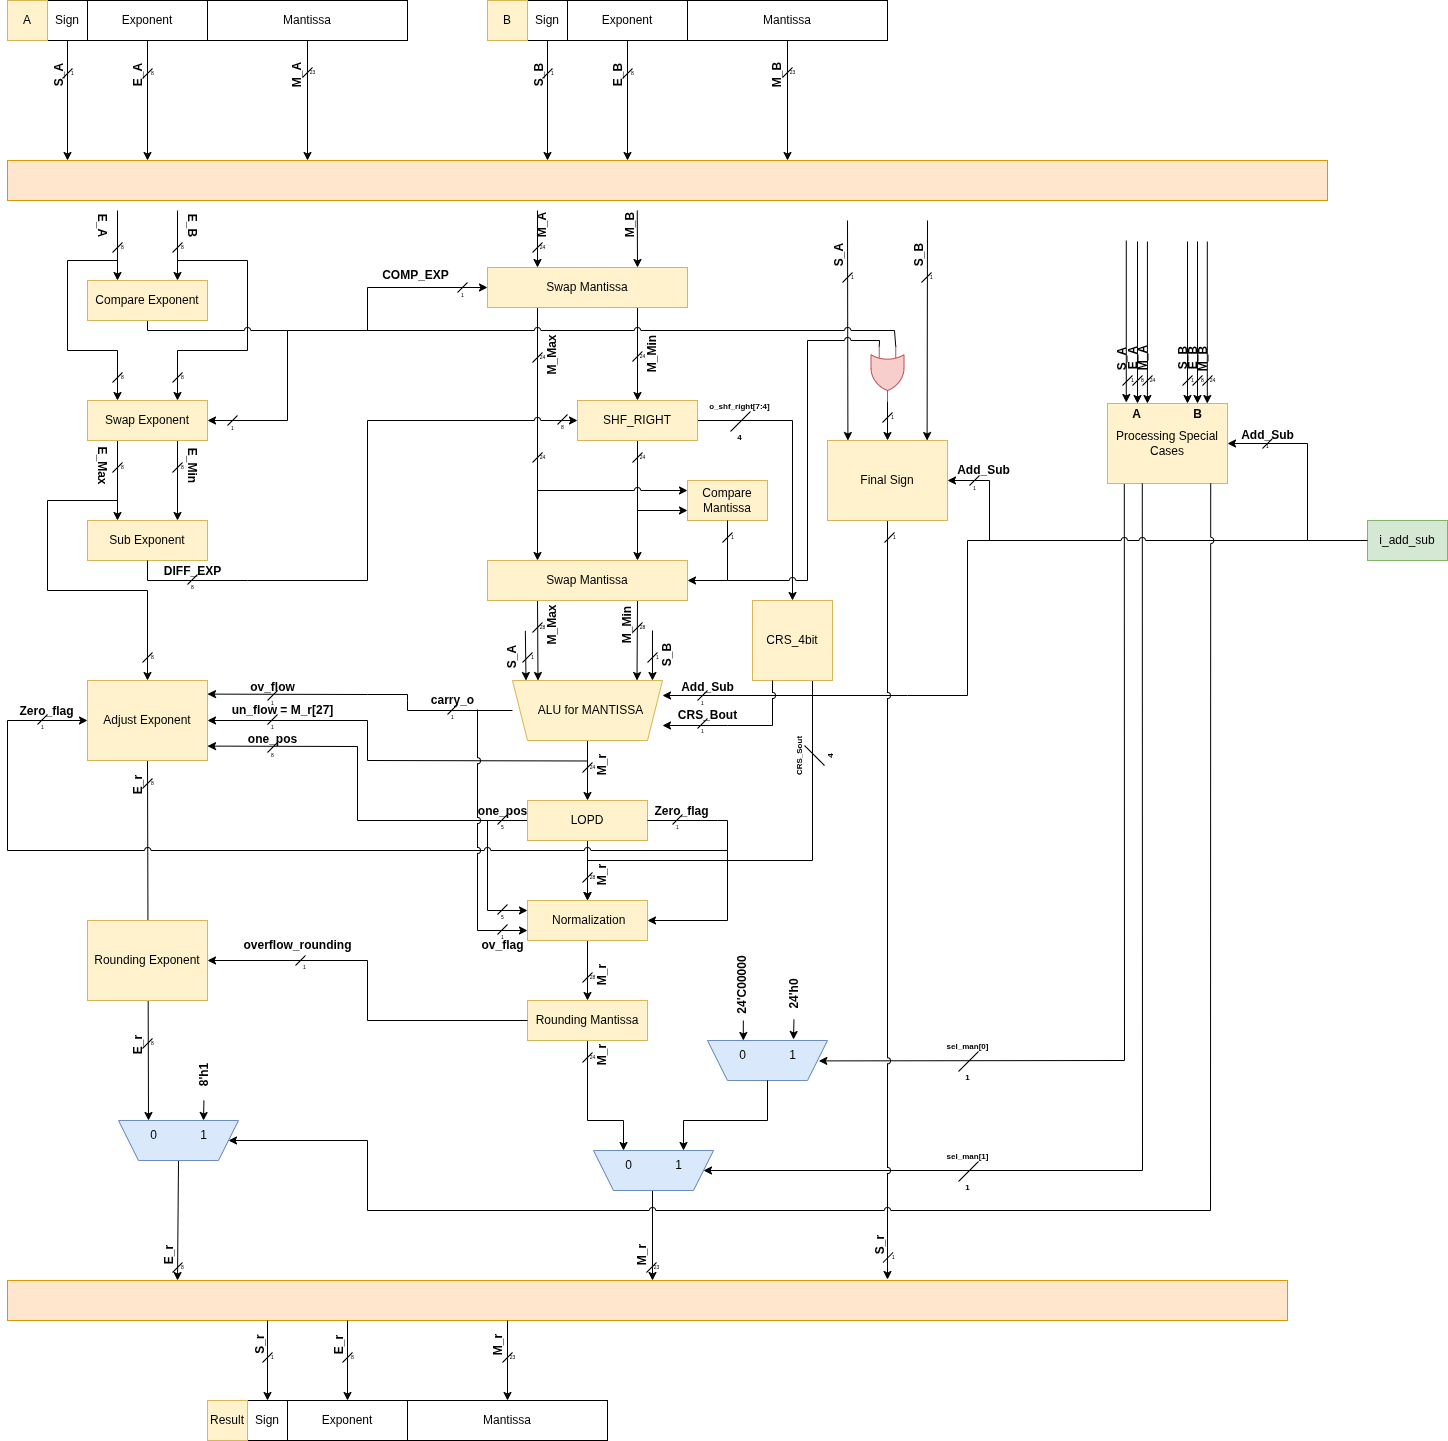
\includegraphics[width=.7\linewidth]{./../Version1/02_rtl/PA_CAL_MEAN/BFP16_ADD/00_spec/BlockDiagram_Overview.png}
	\caption{Bộ thực hiện 2 số Floating Point 32-bit.}
	\label{fig: RTL_BFP16}
\end{figure}



\subsubsection{Bộ tính cộng tích lũy của mảng (PA\_Cal\_Sum)}

\begin{figure}[H]
	\centering
	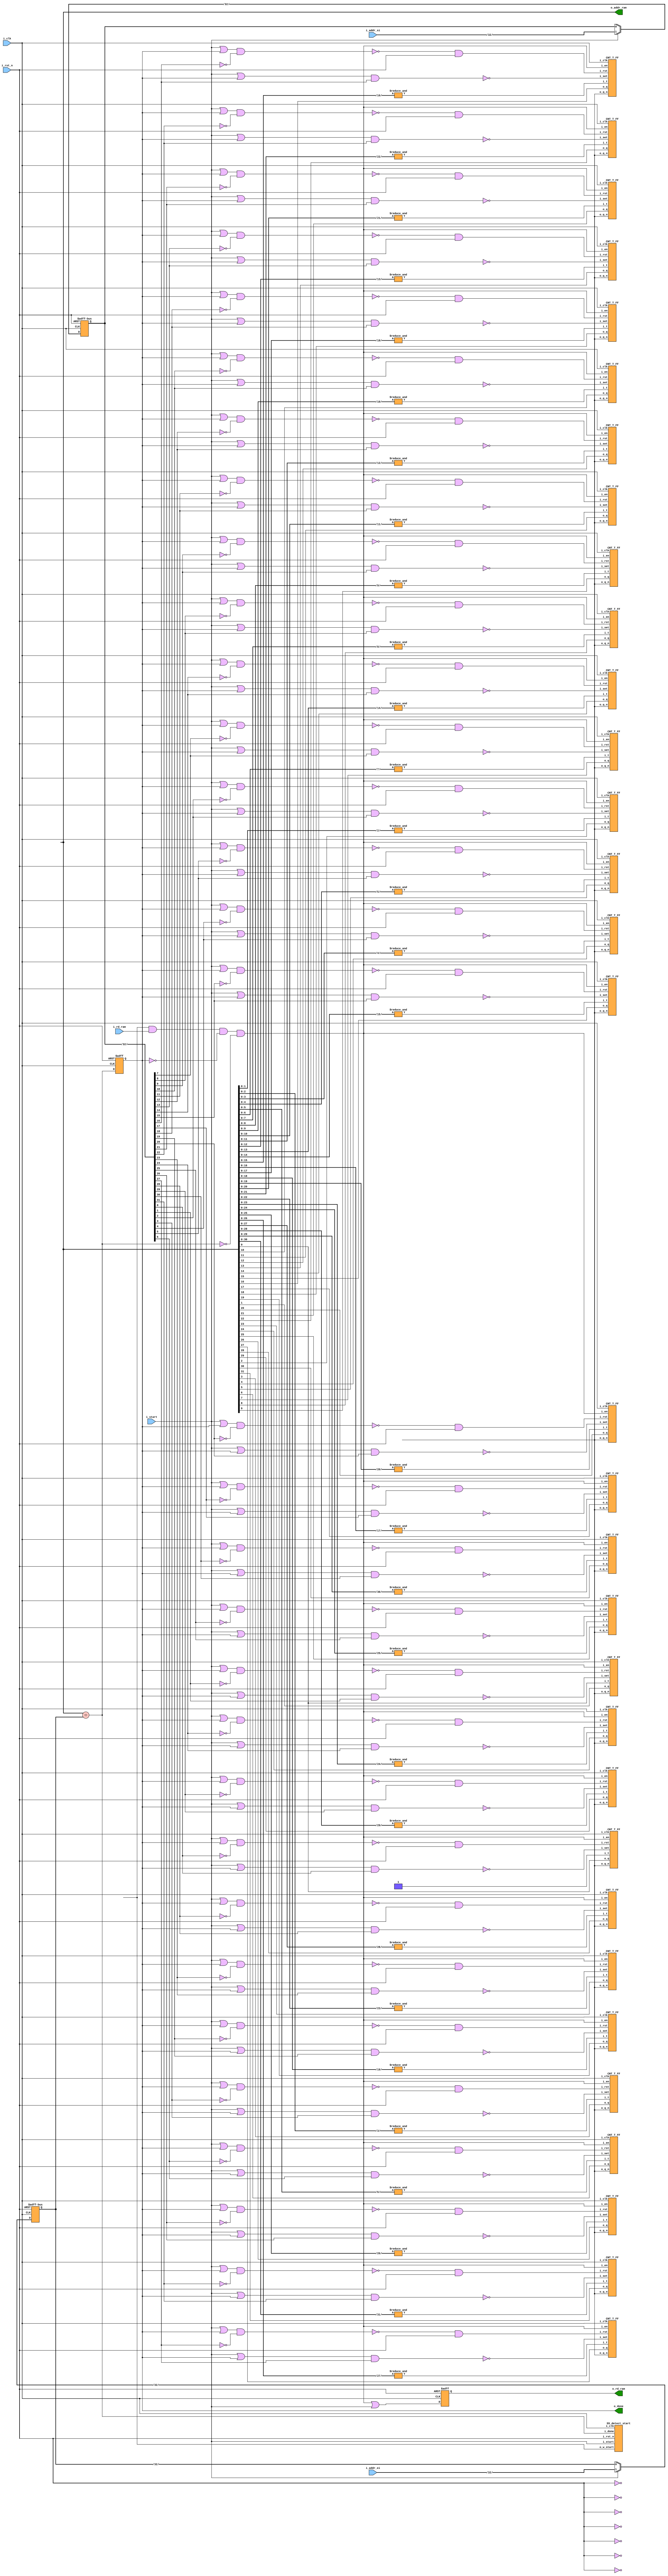
\includegraphics[width=.2\linewidth]{./../Version1/02_rtl/PA_CAL_MEAN/00_spec/PACS_control_address_diagram.png}
	\caption{Bộ điều khiển dữ liệu đọc với Memory Unit.}
\end{figure}

\begin{figure}[H]
	\centering
	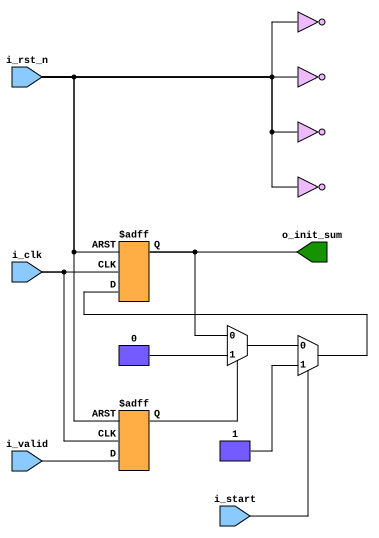
\includegraphics[width=.4\linewidth]{./../Version1/02_rtl/PA_CAL_MEAN/00_spec/PACS_detect_init_data.png}
	\caption{Bộ phát hiện tính hiệu bắt đầu.}
\end{figure}

\begin{figure}[H]
	\centering
	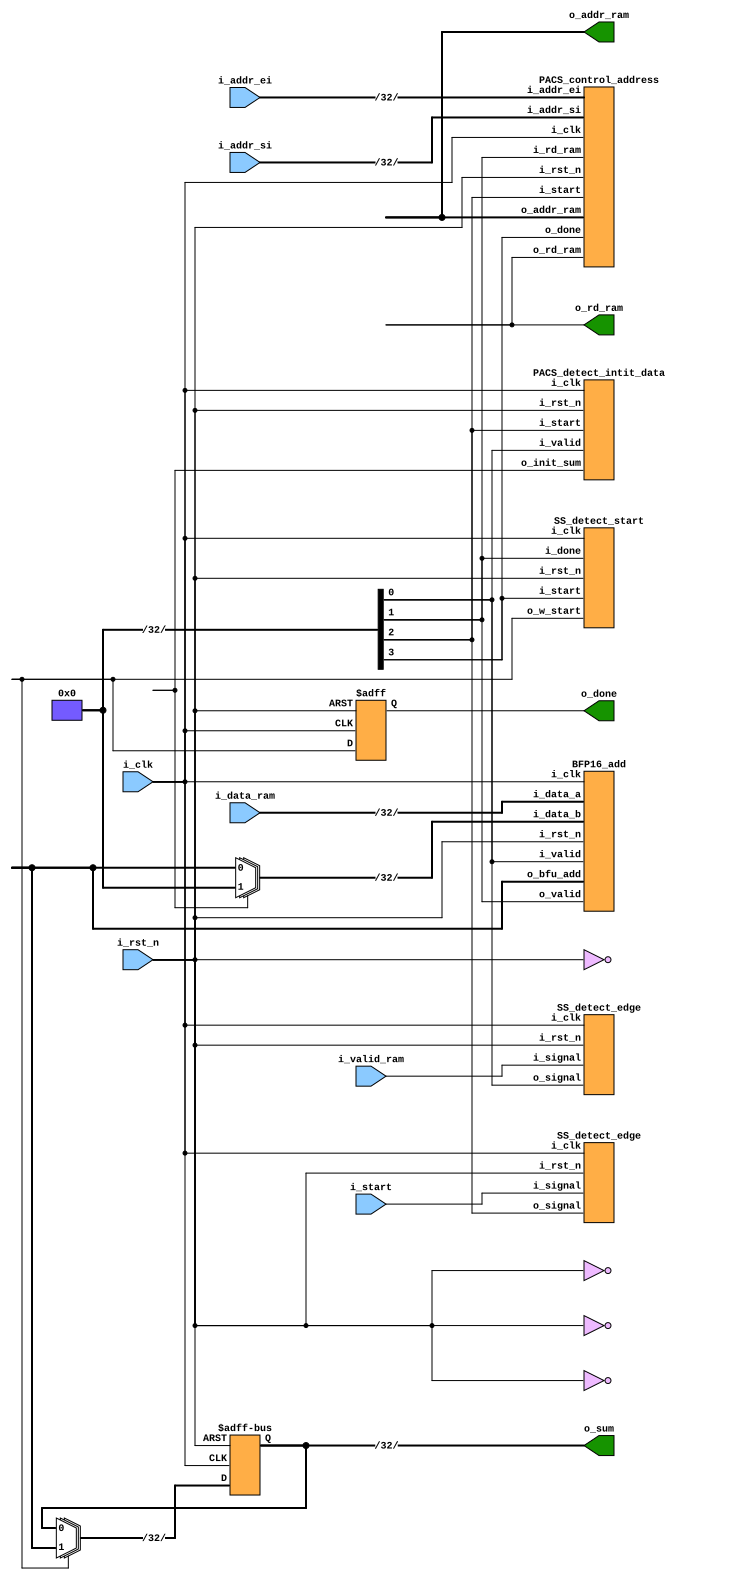
\includegraphics[width=.4\linewidth]{./../Version1/02_rtl/PA_CAL_MEAN/00_spec/PA_cal_sum_diagram.png}
	\caption{Bộ tính cộng số thực (BFP16\_add).}
\end{figure}

\subsubsection{Bộ tính chia số thực (FP32\_div)}

\begin{figure}[H]
	\centering
	\includegraphics[width=.5\linewidth]{./../Version1/02_rtl/PA_CAL_MEAN/BFP16_DIV/00_spec/FPU32_div_diagram.png}
	\caption{Bộ chia số thực.}
\end{figure}

\subsection{Bộ thực hiện partition lại mảng theo giá trị trung bình (PAMEM\_UNIT)}

\subsection{Bộ thực hiện đệ quy cho giải thuật (DI\_UNIT)}

\begin{figure}[H]
	\centering
	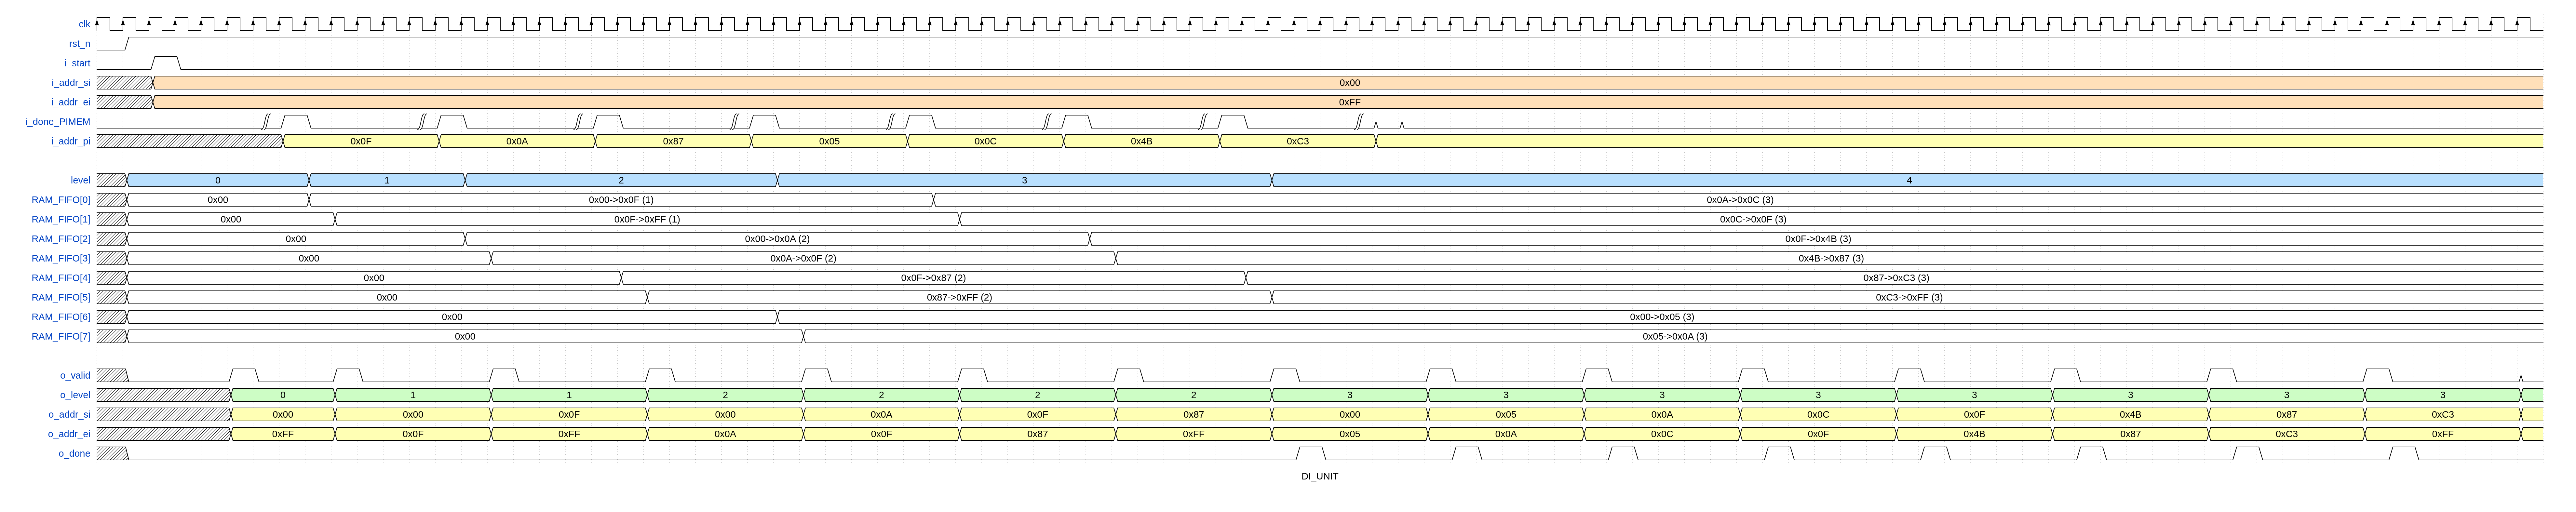
\includegraphics[width=\linewidth]{./../Version1/02_rtl/DI_UNIT/00_spec/WaveDrome_DI_unit.png}
\end{figure}